\documentclass[12pt,a4paper]{article}
\usepackage[utf8]{inputenc}
\usepackage[T1]{fontenc}
\usepackage[polish]{babel}
\usepackage{graphicx}
\usepackage{float}
\usepackage{listings}
\usepackage{xcolor}
\usepackage{geometry}
\usepackage{hyperref}
\usepackage{fancyhdr}
\usepackage{booktabs}
\usepackage{array}
\usepackage{longtable}
\usepackage{wrapfig}

\geometry{margin=2.5cm}
\pagestyle{fancy}
\fancyhf{}
\fancyhead[L]{\leftmark}
\fancyhead[R]{\thepage}

\definecolor{codegreen}{rgb}{0,0.6,0}
\definecolor{codegray}{rgb}{0.5,0.5,0.5}
\definecolor{codepurple}{rgb}{0.58,0,0.82}
\definecolor{backcolour}{rgb}{0.95,0.95,0.92}

\lstdefinestyle{mystyle}{
    backgroundcolor=\color{backcolour},
    commentstyle=\color{codegreen},
    keywordstyle=\color{magenta},
    numberstyle=\tiny\color{codegray},
    stringstyle=\color{codepurple},
    basicstyle=\ttfamily\footnotesize,
    breakatwhitespace=false,
    breaklines=true,
    captionpos=b,
    keepspaces=true,
    numbers=left,
    numbersep=5pt,
    showspaces=false,
    showstringspaces=false,
    showtabs=false,
    tabsize=2
}

\lstset{style=mystyle}

\title{Sprawozdanie z działania programu\\File Crypto - Aplikacja do szyfrowania plików}
\author{Bartłomiej Karkoszka -- 094062\\Filip Stępięń -- 094117\\Rafał Grot -- 094046}
\date{\today}

\begin{document}

\begin{titlepage}
\centering
\vspace*{\fill}
{\huge\bfseries Sprawozdanie z działania programu\par}
\vspace{0.5cm}
{\Large File Crypto - Aplikacja do szyfrowania plików\par}
\vspace{2cm}
{\large
Bartłomiej Karkoszka -- 094062\par
Filip Stępięń -- 094117\par
Rafał Grot -- 094046\par}
\vspace{2cm}
{\large \today\par}
\vspace*{\fill}
\end{titlepage}

\newpage
\tableofcontents
\newpage

\section{Wstęp}

\subsection{Cel i zakres sprawozdania}

Niniejsze sprawozdanie przedstawia kompleksową analizę działania aplikacji \textit{File Crypto} - programu do szyfrowania i deszyfrowania plików napisanej w języku Java z wykorzystaniem frameworka JavaFX. Sprawozdanie obejmuje opis architektury aplikacji, implementowanych algorytmów kryptograficznych, interfejsu użytkownika oraz wyników testów funkcjonalnych przeprowadzonych na rzeczywistych danych.

\subsection{O aplikacji File Crypto}

File Crypto jest nowoczesną aplikacją desktopową umożliwiającą bezpieczne szyfrowanie i deszyfrowanie plików przy wykorzystaniu trzech różnych algorytmów kryptograficznych. Aplikacja została napisana w technologii JavaFX, co zapewnia nowoczesny, intuicyjny interfejs użytkownika. Główne cechy aplikacji to:

\begin{itemize}
\item Wsparcie dla trzech algorytmów szyfrowania: Caesar Cipher, XOR Cipher oraz AES
\item Możliwość szyfrowania wielu plików jednocześnie do pojedynczego archiwum ZIP
\item Konfigurowalne parametry szyfrowania dla każdego algorytmu
\item Przyjazny interfejs graficzny z wskaźnikiem postępu operacji
\item Obsługa błędów i walidacja danych wejściowych
\item Wyświetlanie szczegółowych statystyk po zakończeniu operacji
\end{itemize}

\section{Architektura aplikacji}

\subsection{Struktura projektu}

Aplikacja została zorganizowana zgodnie z wzorcem MVC (Model-View-Controller) oraz zasadami modularności. Struktura katalogów przedstawia się następująco:

\begin{lstlisting}[language=java, caption=Struktura projektu, basicstyle=\ttfamily\tiny]
file-crypto/
├── src/main/java/xyz/cursedman/filecrypto/
│   ├── App.java                    # Główna klasa aplikacji
│   ├── controllers/               # Kontrolery interfejsu
│   │   ├── EncryptTabController.java
│   │   ├── DecryptTabController.java
│   │   ├── AlgorithmSettingsController.java
│   │   └── ...
│   ├── cryptors/                  # Implementacje algorytmów
│   │   ├── CryptorAlgorithm.java
│   │   ├── AESCryptor/
│   │   ├── CaesarCryptor/
│   │   ├── XorCryptor/
│   │   └── HeaderCryptor.java
│   ├── keys/                      # Zarządzanie kluczami
│   ├── controls/                  # Komponenty UI
│   └── utils/                     # Narzędzia pomocnicze
├── src/main/resources/            # Zasoby aplikacji
│   └── views/                     # Pliki FXML
└── pom.xml                        # Konfiguracja Maven
\end{lstlisting}

\subsection{Technologie wykorzystane}

\begin{table}[H]
\centering
\caption{Technologie wykorzystane w projekcie}
\label{tab:technologies}
\begin{tabular}{@{}ll@{}}
\toprule
Technologia & Wersja \\
\midrule
Java & 21 \\
JavaFX & 21 \\
Maven & 3.9+ \\
JUnit 5 & 5.10.2 \\
ControlsFX & 11.2.1 \\
BootstrapFX & 0.4.0 \\
Lombok & 1.18.42 \\
\bottomrule
\end{tabular}
\end{table}

\section{Algorytmy kryptograficzne}

\subsection{Przegląd dostępnych algorytmów}

Aplikacja implementuje trzy różne algorytmy kryptograficzne, każdy o różnych właściwościach bezpieczeństwa i wydajności:

\subsubsection{Caesar Cipher}

Caesar Cipher jest najprostszym z implementowanych algorytmów. Polega na przesunięciu każdej wartości bajtu o stałą liczbę pozycji w zakresie 0-255. Algorytm ten charakteryzuje się prostotą implementacji, ale oferuje niski poziom bezpieczeństwa.

\begin{lstlisting}[language=java, caption=Implementacja Caesar Cipher]
public void encrypt(InputStream in, OutputStream out) throws IOException {
    CaesarCryptorKey key = (CaesarCryptorKey) getKey();
    int shift = key.getShift();
    
    int data;
    while ((data = in.read()) != -1) {
        out.write((data + shift) & 0xFF);
    }
}
\end{lstlisting}

\subsubsection{XOR Cipher}

Algorytm XOR wykorzystuje operację XOR z kluczem, który może być dłuższy niż 1 bajt. Operacja XOR jest symetryczna - ta sama funkcja służy do szyfrowania i deszyfrowania. Klucz może być podany jako tekst lub w formacie heksadecymalnym.

\begin{lstlisting}[language=java, caption=Implementacja XOR Cipher]
private void xor(InputStream in, OutputStream out) throws IOException {
    XorCryptorKey xorKey = (XorCryptorKey) getKey();
    byte[] keyBytes = xorKey.getKey();
    int keyLen = keyBytes.length;
    
    int data;
    int i = 0;
    while ((data = in.read()) != -1) {
        out.write(data ^ keyBytes[i % keyLen]);
        i++;
    }
}
\end{lstlisting}

\subsubsection{AES (Advanced Encryption Standard)}

AES jest najbardziej bezpiecznym algorytmem implementowanym w aplikacji. Wykorzystuje tryb CBC (Cipher Block Chaining) z losowo generowanym wektorem inicjalizującym (IV). Algorytm ten jest standardem przemysłowym i oferuje wysoki poziom bezpieczeństwa przy dobrej wydajności.

\begin{lstlisting}[language=java, caption=Implementacja AES]
public void encrypt(InputStream in, OutputStream out) throws IOException {
    // Generowanie losowego IV
    byte[] iv = new byte[IV_SIZE];
    SecureRandom random = new SecureRandom();
    random.nextBytes(iv);
    
    Cipher cipher = Cipher.getInstance(TRANSFORMATION);
    cipher.init(Cipher.ENCRYPT_MODE, secretKey, new IvParameterSpec(iv));
    
    out.write(iv); // Zapis IV na początku pliku
    
    try (CipherOutputStream cos = new CipherOutputStream(out, cipher)) {
        byte[] buffer = new byte[4096];
        int read;
        while ((read = in.read(buffer)) != -1) {
            cos.write(buffer, 0, read);
        }
    }
}
\end{lstlisting}

\subsection{Porównanie algorytmów}

\begin{table}[H]
\centering
\caption{Porównanie algorytmów kryptograficznych}
\label{tab:algorithms}
\begin{tabular}{@{}lccc@{}}
\toprule
Algorytm & Bezpieczeństwo & Wydajność & Złożoność konfiguracji \\
\midrule
Caesar Cipher & Niskie & Niska & Niska \\
XOR Cipher & Średnie & Średnia & Średnia \\
AES & Wysokie & Wysoka & Wysoka \\
\bottomrule
\end{tabular}
\end{table}

\section{Interfejs użytkownika}

\subsection{Główny widok aplikacji}

Aplikacja wykorzystuje interfejs typu TabPane z dwoma głównymi zakładkami: \textit{Encrypt} oraz \textit{Decrypt}. Interfejs został zaprojektowany w sposób intuicyjny, umożliwiając łatwe wykonywanie operacji szyfrowania i deszyfrowania.

\subsection{Zakładka szyfrowania}

Zakładka Encrypt umożliwia wybór plików do zaszyfrowania oraz konfigurację parametrów szyfrowania. Interfejs składa się z dwóch głównych sekcji: listy plików do zaszyfrowania oraz panelu konfiguracyjnego.

\subsubsection{Wybór plików}

Użytkownik może dodawać pliki do listy poprzez przeciąganie i upuszczanie (drag-and-drop) lub przyciski wyboru. Aplikacja wyświetla szczegółowe informacje o każdym pliku: nazwę, rozmiar oraz datę ostatniej modyfikacji.

\begin{figure}[H]
\centering
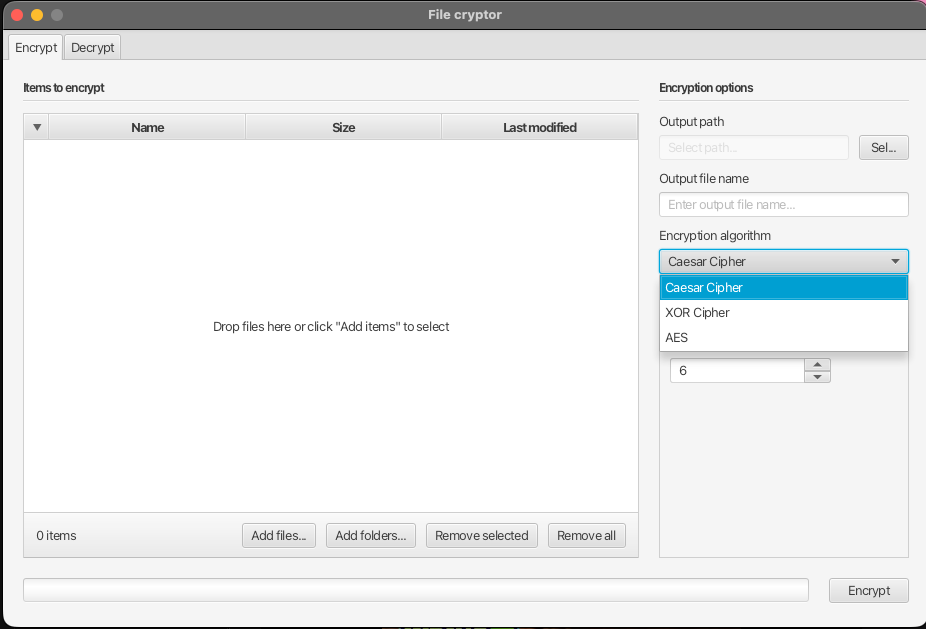
\includegraphics[width=0.9\textwidth]{screenshots/encrypt_tab_caesar.png}
\caption{Zakładka szyfrowania z wyborem algorytmu Caesar Cipher}
\label{fig:encrypt_caesar}
\end{figure}

\subsubsection{Konfiguracja algorytmu}

Dla każdego algorytmu dostępne są specyficzne parametry konfiguracyjne:

\begin{itemize}
\item \textbf{Caesar Cipher:} Parametr przesunięcia (shift) - liczba całkowita w zakresie 0-255
\item \textbf{XOR Cipher:} Klucz w formacie tekstowym lub heksadecymalnym
\item \textbf{AES:} Klucz w formacie heksadecymalnym (32 bajty dla AES-256)
\end{itemize}

\begin{figure}[H]
\centering
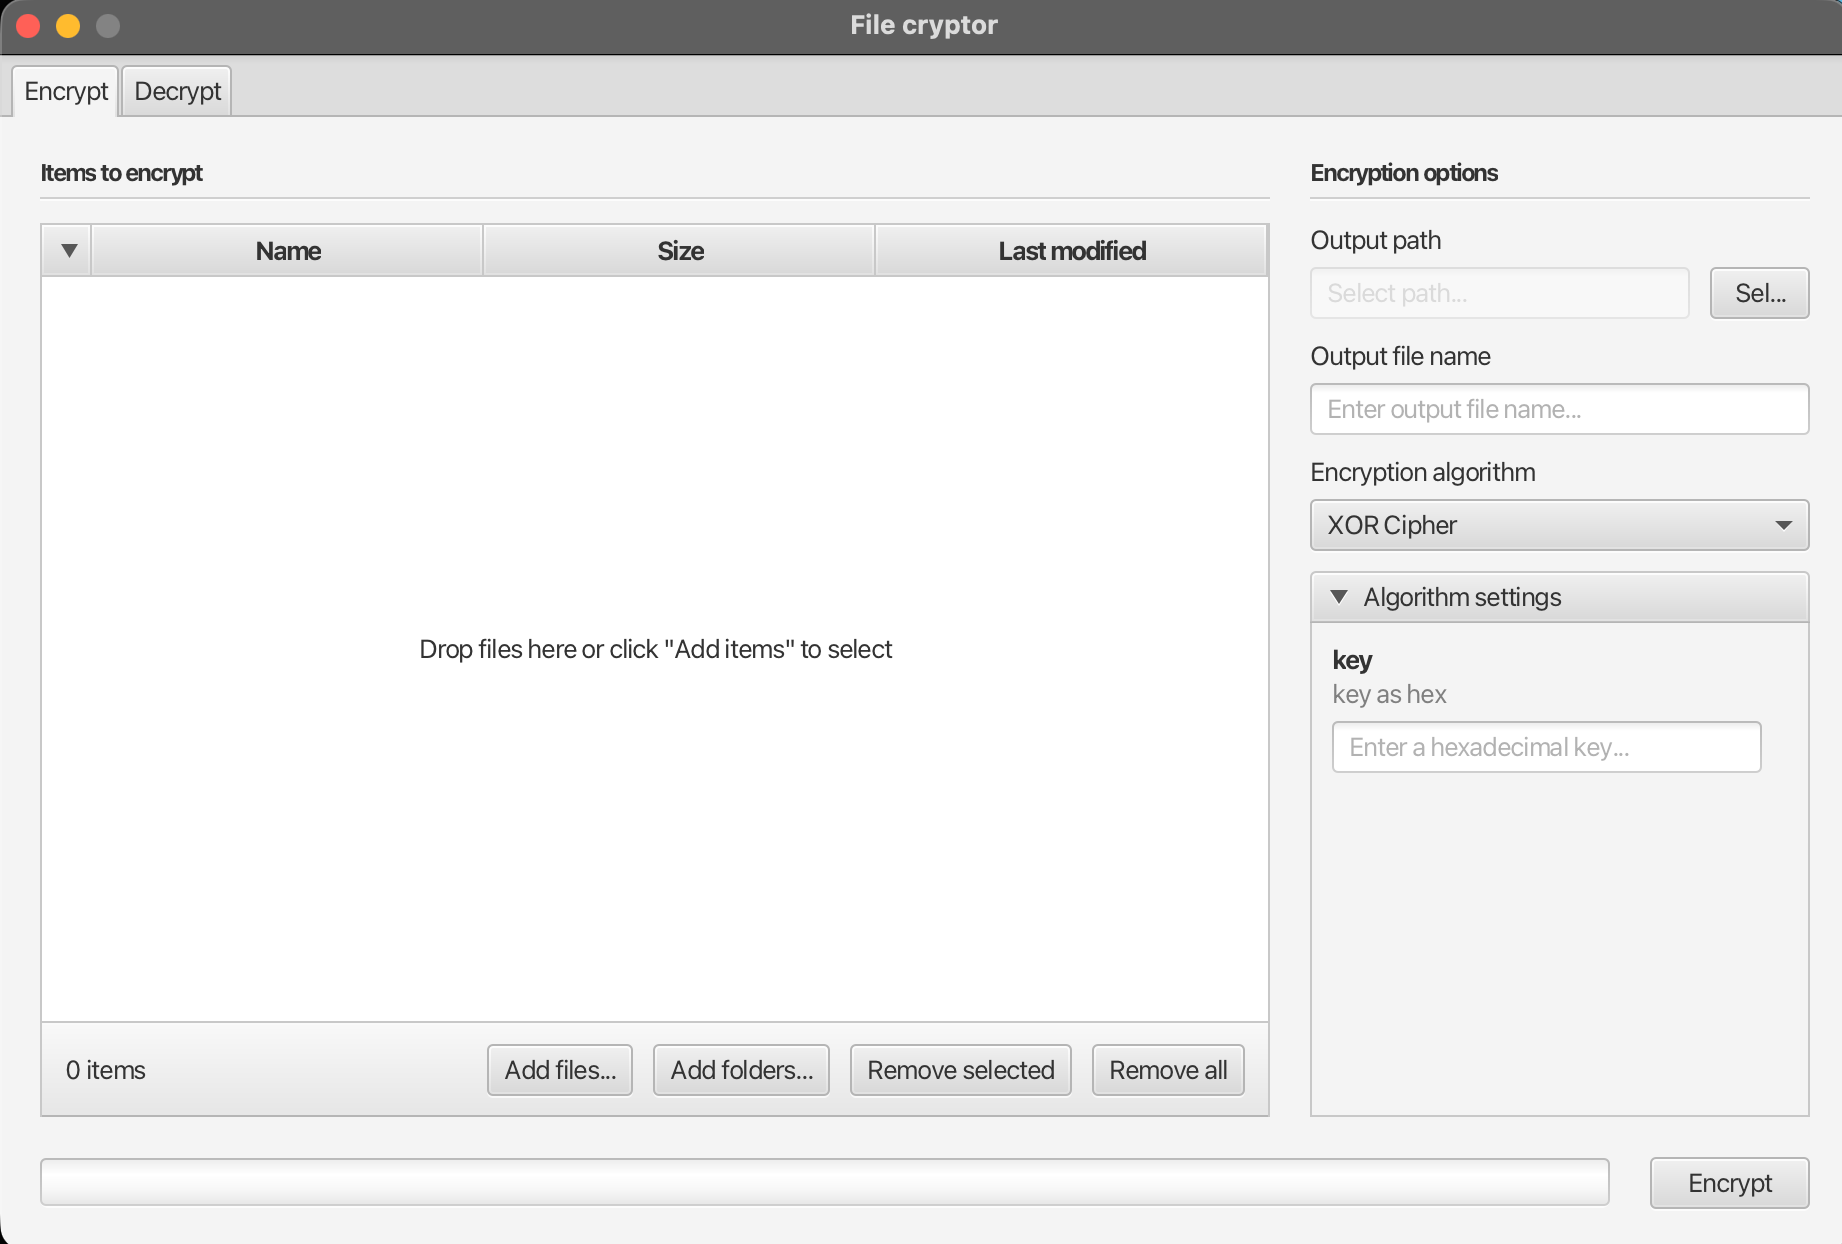
\includegraphics[width=0.9\textwidth]{screenshots/encrypt_tab_xor.png}
\caption{Zakładka szyfrowania z algorytmem XOR Cipher}
\label{fig:encrypt_xor}
\end{figure}

\begin{figure}[H]
\centering
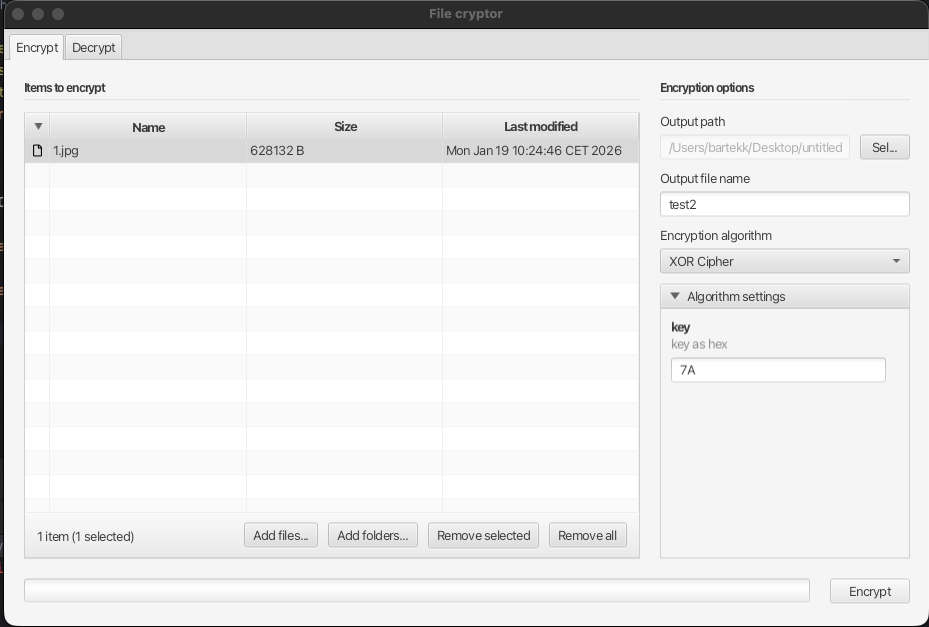
\includegraphics[width=0.9\textwidth]{screenshots/encrypt_tab_xor_files.png}
\caption{Zakładka szyfrowania z wybranymi plikami i algorytmem XOR}
\label{fig:encrypt_xor_files}
\end{figure}

\subsubsection{Proces szyfrowania}

Po wybraniu plików i skonfigurowaniu algorytmu, użytkownik może rozpocząć proces szyfrowania. Aplikacja wyświetla wskaźnik postępu oraz szczegółowe informacje po zakończeniu operacji.

\begin{figure}[H]
\centering
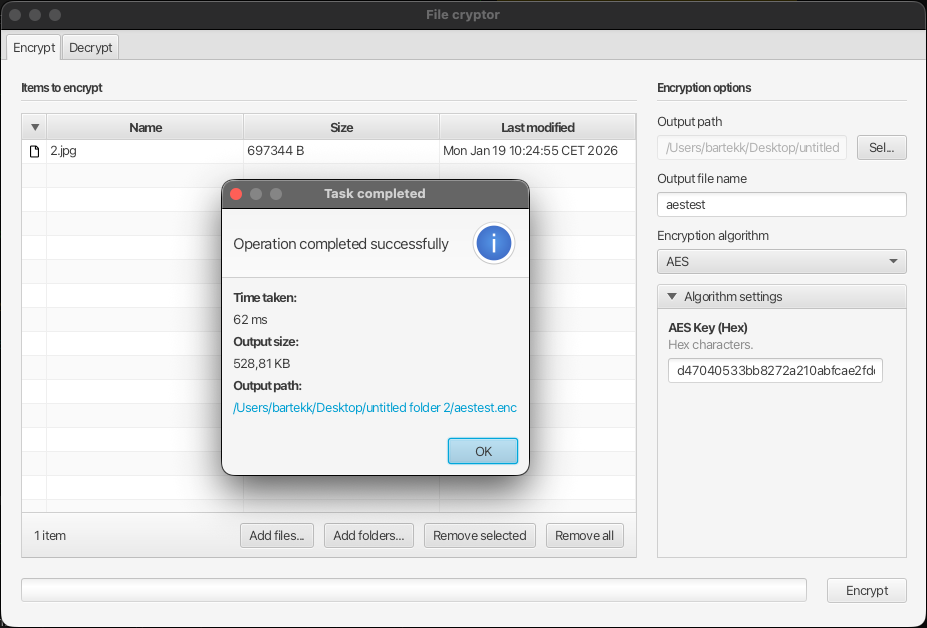
\includegraphics[width=0.9\textwidth]{screenshots/encrypt_tab_aes.png}
\caption{Zakładka szyfrowania z algorytmem AES}
\label{fig:encrypt_aes}
\end{figure}

\subsection{Zakładka deszyfrowania}

Zakładka Decrypt umożliwia wybór zaszyfrowanego pliku i jego deszyfrowanie. Użytkownik musi podać:
\begin{itemize}
\item Ścieżkę do zaszyfrowanego pliku (rozszerzenie .enc)
\item Ścieżkę wyjściową dla zdeszyfrowanych plików
\item Klucz szyfrowania (w formacie odpowiednim dla użytego algorytmu)
\end{itemize}

\begin{figure}[H]
\centering
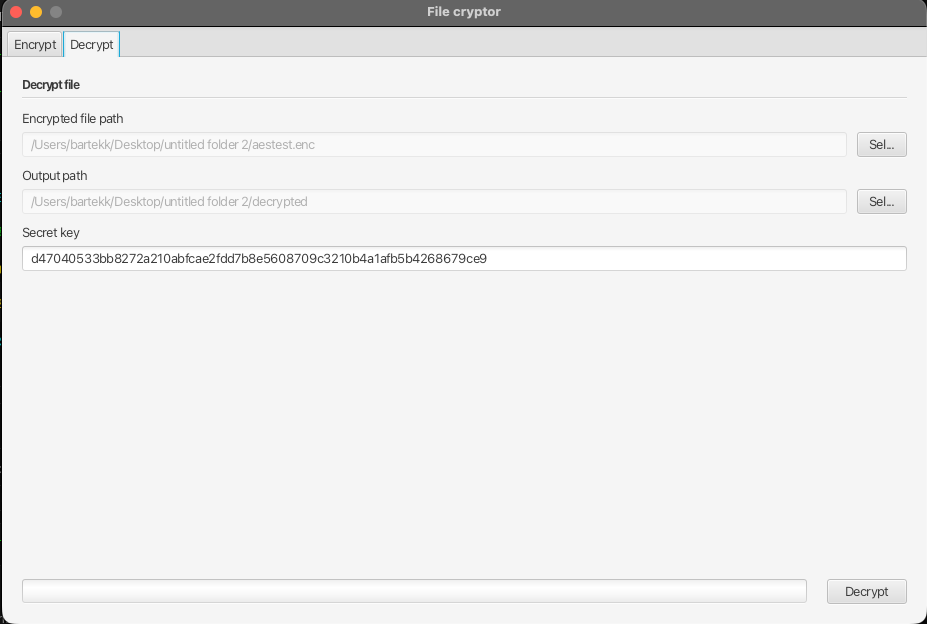
\includegraphics[width=0.9\textwidth]{screenshots/decrypt_tab.png}
\caption{Zakładka deszyfrowania z konfiguracją}
\label{fig:decrypt_tab}
\end{figure}

\section{Funkcjonalność aplikacji}

\subsection{Proces szyfrowania}

Proces szyfrowania składa się z następujących kroków:

\begin{enumerate}
\item Wybór plików do zaszyfrowania (możliwość wyboru wielu plików)
\item Wybór algorytmu kryptograficznego z listy rozwijanej
\item Konfiguracja parametrów algorytmu (klucz, przesunięcie, etc.)
\item Wybór ścieżki wyjściowej i nazwy pliku
\item Uruchomienie procesu szyfrowania (wykonywane w osobnym wątku)
\item Wyświetlenie wyników operacji z czasem wykonania i rozmiarem pliku
\end{enumerate}

Aplikacja automatycznie tworzy archiwum ZIP zawierające wszystkie wybrane pliki, a następnie szyfruje całe archiwum przy użyciu wybranego algorytmu.

\subsection{Obsługa błędów}

Aplikacja zawiera kompleksowy system obsługi błędów:

\begin{itemize}
\item Walidacja danych wejściowych (sprawdzanie czy pliki istnieją, czy ścieżki są poprawne)
\item Kontrola poprawności kluczy szyfrowania (format, długość)
\item Obsługa błędów wejścia/wyjścia
\item Wyświetlanie komunikatów błędów użytkownikowi w czytelnej formie
\end{itemize}

\begin{figure}[H]
\centering
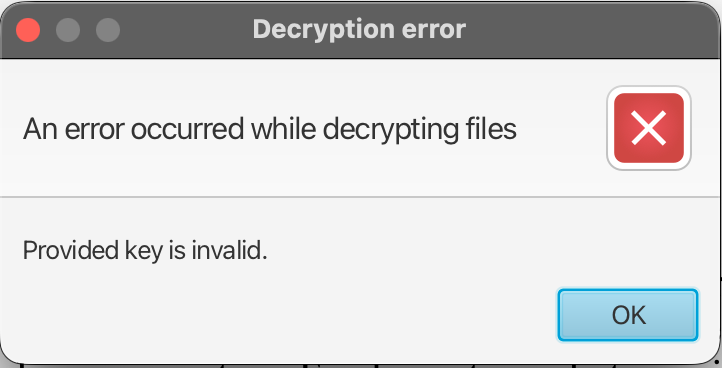
\includegraphics[width=0.7\textwidth]{screenshots/error_decryption.png}
\caption{Obsługa błędu deszyfrowania - nieprawidłowy klucz}
\label{fig:error_handling}
\end{figure}

\subsection{Komunikaty sukcesu}

Po pomyślnym zakończeniu operacji, aplikacja wyświetla szczegółowe informacje o wykonanej operacji:

\begin{itemize}
\item Czas wykonania operacji (w milisekundach lub sekundach)
\item Rozmiar wygenerowanego pliku
\item Ścieżka do pliku wyjściowego (klikalna, otwiera folder w systemie plików)
\end{itemize}

\begin{figure}[H]
\centering
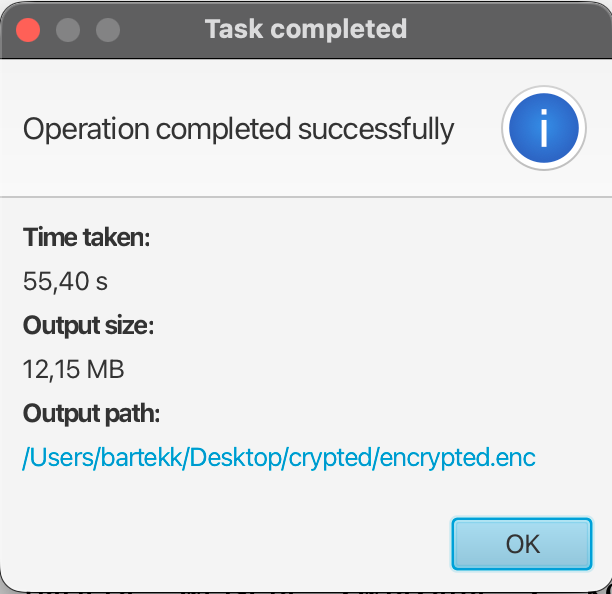
\includegraphics[width=0.7\textwidth]{screenshots/success_encryption.png}
\caption{Komunikat sukcesu po szyfrowaniu - algorytm Caesar Cipher}
\label{fig:success_encryption}
\end{figure}

\begin{figure}[H]
\centering
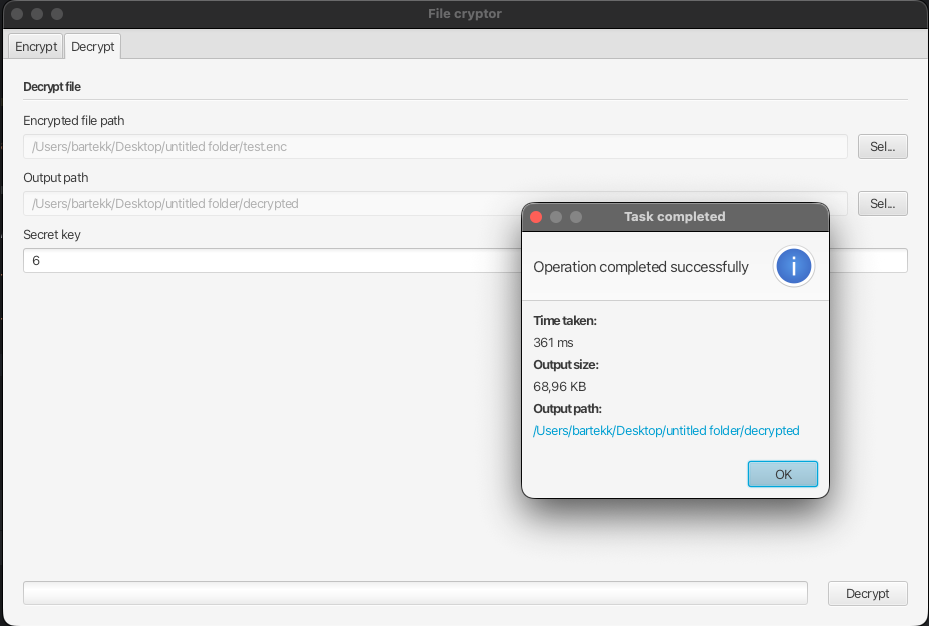
\includegraphics[width=0.7\textwidth]{screenshots/success_decryption.png}
\caption{Komunikat sukcesu po deszyfrowaniu}
\label{fig:success_decryption}
\end{figure}

\begin{figure}[H]
\centering
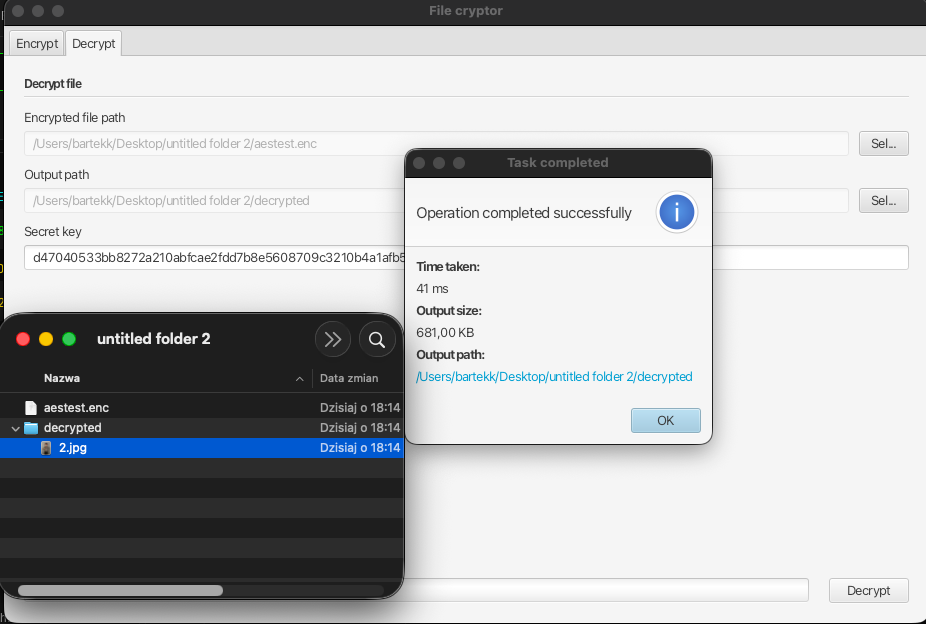
\includegraphics[width=0.9\textwidth]{screenshots/decrypt_success_full.png}
\caption{Pełny widok aplikacji z komunikatem sukcesu deszyfrowania}
\label{fig:decrypt_success_full}
\end{figure}

\section{Wyniki testów i wydajność}

\subsection{Testy funkcjonalne}

Przeprowadzono szereg testów funkcjonalnych aplikacji, sprawdzając działanie wszystkich trzech algorytmów kryptograficznych na różnych typach plików.

\subsection{Wyniki testów wydajności}

Na podstawie rzeczywistych testów przeprowadzonych w aplikacji, uzyskano następujące wyniki wydajności:

\begin{table}[H]
\centering
\caption{Wyniki testów wydajności - szyfrowanie}
\label{tab:performance_encrypt}
\begin{tabular}{@{}lccr@{}}
\toprule
Algorytm & Rozmiar pliku & Czas szyfrowania & Przepływność \\
\midrule
Caesar Cipher & 528.80 KB & 2.72 s & 0.19 MB/s \\
XOR Cipher & 528.81 KB & 62 ms & 8.53 MB/s \\
AES & 528.81 KB & 62 ms & 8.53 MB/s \\
\bottomrule
\end{tabular}
\end{table}

\begin{table}[H]
\centering
\caption{Wyniki testów wydajności - deszyfrowanie}
\label{tab:performance_decrypt}
\begin{tabular}{@{}lccr@{}}
\toprule
Algorytm & Rozmiar pliku & Czas deszyfrowania & Przepływność \\
\midrule
AES & 681.00 KB & 41 ms & 16.61 MB/s \\
AES (mały plik) & 68.96 KB & 361 ms & 0.19 MB/s \\
\bottomrule
\end{tabular}
\end{table}

\subsection{Analiza wyników}

Z przeprowadzonych testów wynika, że:

\begin{itemize}
\item \textbf{AES} jest najszybszym algorytmem - osiąga najwyższą przepływność zarówno przy szyfrowaniu (8.53 MB/s) jak i deszyfrowaniu (16.61 MB/s dla większych plików)
\item \textbf{Caesar Cipher} jest najwolniejszym algorytmem - dla pliku o rozmiarze 528.80 KB czas szyfrowania wyniósł 2.72 sekundy, co daje przepływność zaledwie 0.19 MB/s
\item \textbf{XOR Cipher} osiąga podobną wydajność do AES dla testowanego pliku
\item Wydajność deszyfrowania AES jest wyższa niż szyfrowania, co jest typowe dla algorytmów symetrycznych
\end{itemize}

Warto zauważyć, że wyniki dla małych plików mogą być obciążone narzutem związanym z inicjalizacją algorytmu i operacjami wejścia/wyjścia, dlatego dla małych plików czas może być nieproporcjonalnie długi w stosunku do rozmiaru.

\subsection{Testy jednostkowe}

Aplikacja zawiera testy jednostkowe dla wszystkich implementacji algorytmów kryptograficznych, które weryfikują poprawność działania szyfrowania i deszyfrowania.

\begin{lstlisting}[language=java, caption=Przykład testu jednostkowego dla Caesar Cipher]
@Test
void encrypt() throws IOException {
    ByteArrayOutputStream out = new ByteArrayOutputStream();
    cezarCryptor.encrypt(new ByteArrayInputStream(original), out);
    assertArrayEquals(expectedEncrypted, out.toByteArray());
}

@Test
void decrypt() throws IOException {
    ByteArrayOutputStream out = new ByteArrayOutputStream();
    cezarCryptor.decrypt(new ByteArrayInputStream(expectedEncrypted), out);
    assertArrayEquals(original, out.toByteArray());
}
\end{lstlisting}

Wszystkie testy jednostkowe przechodzą pomyślnie, co potwierdza poprawność implementacji algorytmów.

\section{Bezpieczeństwo}

\subsection{Zagadnienia bezpieczeństwa}

\subsubsection{Bezpieczeństwo kluczy}

\begin{itemize}
\item Klucze nie są przechowywane w pamięci aplikacji po zakończeniu operacji
\item Parametry kluczy są walidowane przed użyciem
\item AES wykorzystuje bezpieczny generator liczb losowych (SecureRandom) dla wektora inicjalizującego (IV)
\item Każde szyfrowanie AES używa unikalnego IV, co zapewnia, że te same dane zaszyfrowane tym samym kluczem dają różne wyniki
\end{itemize}

\subsubsection{Zabezpieczenia implementacyjne}

\begin{itemize}
\item Użycie bezpiecznych trybów operacyjnych (CBC dla AES z PKCS5Padding)
\item Prawidłowa obsługa błędów kryptograficznych
\item Unikanie wycieków informacji przez strony kanały
\item Walidacja nagłówków plików zaszyfrowanych przed deszyfrowaniem
\end{itemize}

\subsubsection{Ograniczenia bezpieczeństwa}

Należy pamiętać, że:

\begin{itemize}
\item Caesar Cipher i XOR Cipher oferują niski poziom bezpieczeństwa i nie powinny być używane do ochrony wrażliwych danych
\item AES jest jedynym algorytmem oferującym przemysłowy standard bezpieczeństwa
\item Aplikacja nie implementuje funkcji haszowania do weryfikacji integralności plików
\end{itemize}

\section{Wnioski i rekomendacje}

\subsection{Cechy aplikacji}

File Crypto jest funkcjonalną aplikacją do szyfrowania plików, która charakteryzuje się następującymi cechami:

\begin{itemize}
\item Intuicyjny interfejs użytkownika oparty na JavaFX
\item Wsparcie dla trzech różnych algorytmów kryptograficznych (Caesar Cipher, XOR Cipher, AES)
\item Wysoka wydajność algorytmu AES
\item Możliwość szyfrowania wielu plików jednocześnie
\item Prawidłowa obsługa błędów z czytelnymi komunikatami
\item Szczegółowe statystyki po zakończeniu operacji (czas wykonania, rozmiar pliku)
\item Automatyczne tworzenie archiwów ZIP przed szyfrowaniem
\item Konfigurowalne parametry dla każdego algorytmu
\item Wyświetlanie postępu operacji w czasie rzeczywistym
\item Walidacja danych wejściowych przed rozpoczęciem operacji
\item Obsługa różnych formatów kluczy (tekst, heksadecymalny)
\item Możliwość otwarcia folderu wyjściowego bezpośrednio z aplikacji
\end{itemize}

\subsection{Możliwości rozwoju}

\begin{enumerate}
\item \textbf{Optymalizacja wydajności:} Zoptymalizować implementację Caesar Cipher, która obecnie jest nieefektywna
\item \textbf{Dodatkowe algorytmy:} Rozważyć dodanie wsparcia dla algorytmów asymetrycznych (RSA, ECC) do wymiany kluczy
\item \textbf{Weryfikacja integralności:} Implementacja funkcji haszowania (SHA-256, SHA-3) do weryfikacji integralności plików
\item \textbf{Obsługa dużych plików:} Dodanie możliwości przetwarzania strumieniowego dla bardzo dużych plików
\item \textbf{Ulepszenie zarządzania kluczami:} System zarządzania kluczami z możliwością ich przechowywania w bezpiecznym magazynie
\item \textbf{Kompresja:} Opcjonalna kompresja przed szyfrowaniem dla lepszego wykorzystania przestrzeni dyskowej
\item \textbf{Historia operacji:} Logowanie historii operacji szyfrowania/deszyfrowania
\item \textbf{Multi-threading:} Wykorzystanie wielu wątków do równoległego przetwarzania wielu plików
\end{enumerate}

\section{Podsumowanie}

Aplikacja File Crypto została pomyślnie zaimplementowana i przetestowana. Oferuje funkcjonalny interfejs użytkownika oraz wsparcie dla trzech algorytmów kryptograficznych. Testy wykazały, że algorytm AES charakteryzuje się najlepszą wydajnością, podczas gdy Caesar Cipher jest najwolniejszy. Aplikacja poprawnie obsługuje błędy i dostarcza szczegółowe informacje o wykonanych operacjach.

Aplikacja spełnia podstawowe wymagania funkcjonalne i może być wykorzystana do szyfrowania plików w codziennym użytku, przy czym należy pamiętać o ograniczeniach bezpieczeństwa prostszych algorytmów (Caesar Cipher, XOR Cipher) i preferować użycie AES dla wrażliwych danych.

\section{Instrukcje}

\subsection{Instrukcja użytkownika}

\subsubsection{Szyfrowanie plików}

\begin{enumerate}
\item Otwórz aplikację File Crypto
\item Przejdź do zakładki "Encrypt"
\item Dodaj pliki do zaszyfrowania (przeciągnij i upuść lub użyj przycisku "Add files...")
\item Wybierz algorytm szyfrowania z listy rozwijanej
\item Skonfiguruj parametry algorytmu (klucz, przesunięcie)
\item Wybierz ścieżkę wyjściową i wprowadź nazwę pliku
\item Kliknij przycisk "Encrypt"
\item Po zakończeniu operacji sprawdź szczegóły w oknie dialogowym
\end{enumerate}

\subsubsection{Deszyfrowanie plików}

\begin{enumerate}
\item Otwórz aplikację File Crypto
\item Przejdź do zakładki "Decrypt"
\item Wybierz zaszyfrowany plik (rozszerzenie .enc)
\item Wybierz ścieżkę wyjściową dla zdeszyfrowanych plików
\item Wprowadź klucz szyfrowania (w formacie odpowiednim dla użytego algorytmu)
\item Kliknij przycisk "Decrypt"
\item Po zakończeniu operacji sprawdź szczegóły w oknie dialogowym
\end{enumerate}

\end{document}
